\documentclass[a4paper,12pt]{article}
\usepackage[utf8]{inputenc}
\usepackage{graphicx}
%  Русский язык
\usepackage{multirow}
\usepackage{wrapfig}
\usepackage[T2A]{fontenc}			% кодировка
\usepackage[utf8]{inputenc}			% кодировка исходного текста
\usepackage[english,russian]{babel}	% локализация и переносы

\usepackage{indentfirst} %Красная строка
\usepackage[a4paper,top=1.3cm,bottom=2cm,left=1.5cm,right=1.5cm,marginparwidth=0.5cm]{geometry}
\usepackage[usenames]{color}
\usepackage{colortbl}
\usepackage{csvsimple}
\usepackage{siunitx}
\usepackage{graphicx}
\graphicspath{ {images/} }
\usepackage{tikz}
\usepackage{pgfplots}

\usepackage{amsmath}
\usepackage{floatflt}
\usepackage[left=20mm, top=20mm, right=20mm, bottom=20mm, footskip=10mm]{geometry}

\usepackage{multicol}
\setlength{\columnsep}{2cm}

\usepackage{multicol}
\setlength{\columnsep}{2cm}
\usepackage{hyperref}


% Заметки
\usepackage{todonotes}

% Математика
\usepackage{amsmath,amsfonts,amssymb,amsthm,mathtools} 
\usepackage{hyperref}

\renewcommand{\AA}{\ensuremath{\mathring{A}}}

\begin{document}
\def\figurename{Рисунок}
\begin{titlepage}
\begin{center}
    {\large МОСКОВСКИЙ ФИЗИКО-ТЕХНИЧЕСКИЙ ИНСТИТУТ (НАЦИОНАЛЬНЫЙ ИССЛЕДОВАТЕЛЬСКИЙ УНИВЕРСИТЕТ)}
\end{center}
\begin{center}
    {\largeФизтех-школа биологической и медицинской физики}
\end{center}

\vspace{1cm}
{\huge
\begin{center}
    {\bf Лабораторная работа по общей физике}\\
    \vspace{0.5cm}
    Интерференция электромагнитных волн миллиметрового диапазона 
\end{center}
}

\vspace{4cm}
\begin{flushright}
{\LARGE Выполнила студентка группы Б06-103:\\ Фитэль Алена \\}

\end{flushright}
\vspace{9cm}
\begin{center}
    Долгопрудный, 2023 г.
\end{center}
\end{titlepage}
\newpage
\section{Введение}


\textbf{Цели работы:}

\item Изучение интерференции электромагнитных волн миллиметрового диапазона с применением двух оптических интерференционных схем, экспериментальное определение длины волны излучения и показателя преломления диэлектрика.
\textbf{В работе используются:} 

\item приёмно-передающая система радиоволн миллиметрового диапазона, металлические зеркала, микрометрический винт, проволочная решётка, пластина из диэлектрика.
\section{Теоретические положения}
Если в некоторой точке пространства происходит суперпозиция двух когерентных одинаково поляризованных волн с интенсивностями $I_1$ и $I_2$ и с разностью фаз $\varphi$, то интенсивность $I$ результирующего колебания определяется соотношением 
\begin{equation}
    I = I_1 + I_2 + 2\sqrt{I_1 I_2}\cos \varphi
\end{equation}
Интенсивность максимальна при $\varphi = 2\pi m$, минимальна при $\varphi = (2m+1)\pi$ ($m = 0, 1, 2, ...$ - порядок интерференции).

\section{Экспериментальная установка}
Источником миллиметровых волн является генератор на клистроне — специальной лампе, генерирующей сверхвысокочастотные колебания. Из клистрона энергия волны подается в прямоугольный волновод. Волноводом называется полая металлическая труба, используемая в СВЧ-диапазоне волн для передачи энергии. Клистрон возбуждает в волноводе
электромагнитную волну, которая распространяется вдоль волновода и с помощью рупорной антенны излучается в пространство. Задача антенны заключается в том, чтобы сделать излучение более направленным. Направленность антенны характеризуют шириной её диаграммы направленности. Чем шире раскрыв рупорной
антенны, тем уже ее диаграмма направленности. \par
Отражённое от препятствия электромагнитное излучение, попадая в рупорную антенну приемника, распространяется по волноводу, в котором имеется детектор высокочастотных колебаний,
работающий в квадратичном режиме. Поэтому ток детектора пропорционален интенсивности I волны, попадающей в приемную антенну. Сигнал с выхода детектора усиливается и измеряется микровольтметром. Принципиальная схема приёмно-передающего тракта представлена на рис. 1.

\begin{figure}[h]
    \centering
    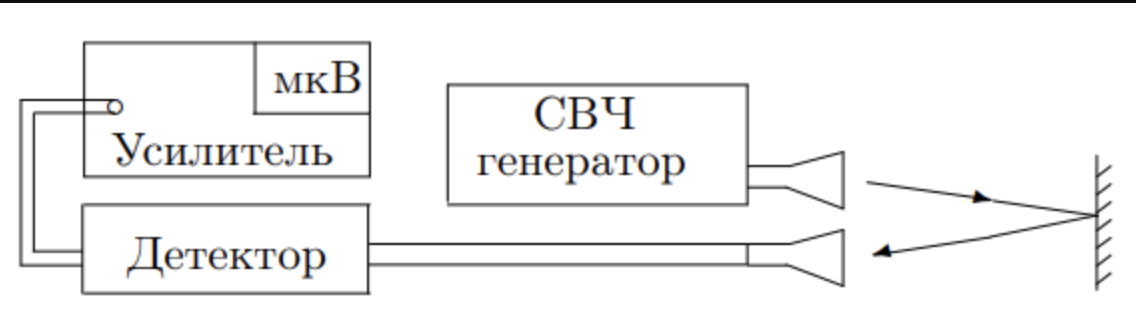
\includegraphics[width=12cm]{pic 1.PNG}
    \caption{Приёмно-передающая система СВЧ-диапазона}
    \label{fig:vac}
\end{figure}

Применяемый в настоящей работе передатчик излучает линейно поляризованную волну, электрический вектор \textbf{E} которой перпендикулярен широкой стенке волновода. Приемник также может принимать только линейно поляризованную волну. Для установления связи в системе, изображенной на рис. 1, необходимо, чтобы широкие стенки волноводов передатчика и приемника были параллельны друг другу.
Если одну из антенн повернуть относительно луча на некоторый угол $\alpha$, интенсивность принимаемого сигнала будет изменяться по \textit{закону Малюса}
\begin{equation}
    I = I_0 \cos^2 \alpha
\end{equation}

\begin{figure}[h]
\begin{center}
\begin{minipage}[h]{0.45\linewidth}
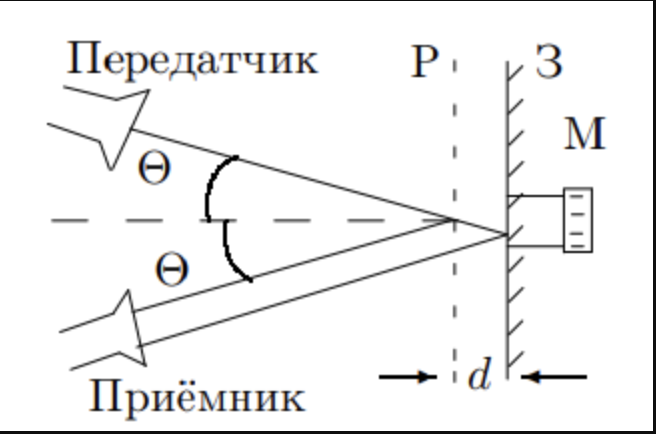
\includegraphics[width=1\linewidth]{pic 2.PNG}
\caption{Интерференция волн СВЧ в плоскопараллельной пластине} %% подпись к рисунку
\label{ris:experimoriginal} %% метка рисунка для ссылки на него
\end{minipage}
\hfill 
\begin{minipage}[h]{0.45\linewidth}
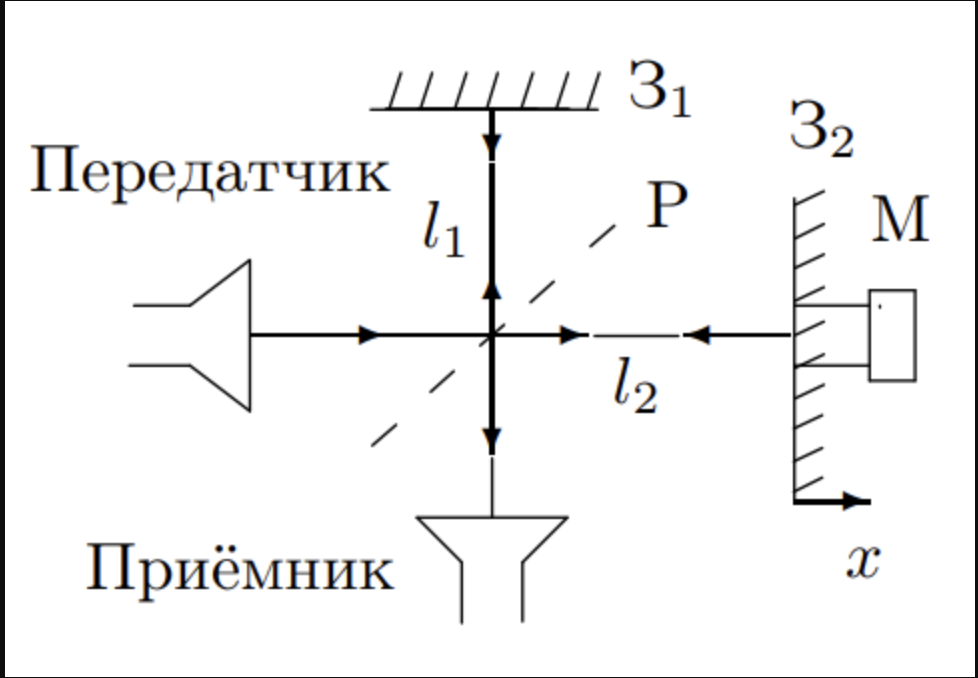
\includegraphics[width=1\linewidth]{pic 3.PNG}
\caption{Интерферометр Майкельсона на СВЧ}
\label{ris:experimcoded}
\end{minipage}
\end{center}
\end{figure}

\subsection{Интерференция радиоволн, отражённых от зеркала и решётки}
Схема установки, используемой для этого опыта, приведена на рис. 2. \par
Металлическое зеркало З и проволочная решетка Р устанавливаются на некотором расстоянии d
друг от друга с помощью специальных фиксаторов. Приемная и передающая антенны располагаются
симметрично, так чтобы в приемник попадала отраженная волна.
Волна, излучаемая передающей антенной, частично отражается от решетки, а частично проходит через нее и отражается от зеркала. Зеркало может перемещаться при помощи микрометрического винта. \par 
Между волнами, отраженными от решетки и от зеркала, возникает разность хода, равная
\begin{equation}
    \triangle = 2 d \cos \theta.
\end{equation}
При изменении разности хода (при изменении d) интенсивность волны в точке приема изменяется в соответствии с формулой (1)

\subsection{Интерферометр Майкельсона}
В этом опыте используется установка, моделирующая оптический интерферометр Майкельсона (рис. 3). Зеркала З1 и З2 располагаются перпендикулярно осям
передающей и приемной антенн, которые в свою очередь должны быть взаимно перпендикулярны. Решетка Р располагается на пересечении осей под углом 45◦ к ним. Волна от передающей антенны
расщепляется на решетке на две волны, распространяющиеся в направлении зеркал З1 и З2. После отражения от зеркал обе волны
возвращаются к решетке. Каждая из этих волн после вторичного расщепления на решетке Р частично попадает в приемную антенну. \par

Разность хода ∆ возникает вследствие различия в расстояниях
$l_1$ и $l_2$ между решеткой Р и зеркалами З1 и З2:
\begin{equation}
    \triangle = 2 (l_2 - l_1).
\end{equation}

При изменении длины одного из плеч интерферометра (при перемещении соответствующего зеркала) интенсивность в точке
приема изменяется в соответствии с формулой (1). \par

Если на пути одного из лучей поставить пластинку толщиной $d_0$ с диэлектрической проницаемостью $\varepsilon$, разность хода изменится
на величину $2 d_0 (n−1)$, где $n = \sqrt{\varepsilon}$ —
показатель преломления вещества,
из которого сделана пластинка. Это
приводит к изменению интенсивности в точке приема. Пусть в точке приема до внесения пластинки наблюдался интерференционный максимум. Для того чтобы получить тот же максимум при наличии пластинки, нужно зеркало свободного плеча интерферометра (плеча, в котором нет пластинки) отодвинуть на расстояние $\triangle x_0$, определяемое выражением
\begin{equation}
    \triangle x_0 = d_0 (n-1).
\end{equation}
Зная $\triangle x_0$, можно определить показатель преломления.

\section{Ход работы}
\subsection{Проверка закона Малюса}
 Расположим рупоры как показано на рис. 2, настроим установку на максимум интенсивности. Снимем зависимость уровня сигнала $I$ от угла поворота $\alpha$ приёмной антенны относительно луча. Результаты занесем в Таблицу 1). Построим график соответствующей зависимости. Как видно из графика, закон Малюса действительно выполняется.


\begin{table}[h!]
\centering
\begin{tabular}{|l|r|r|r|}
\hline
\textbf{\textbf{}} & \multicolumn{1}{l|}{\textbf{\alpha,}} & \multicolumn{1}{l|}{\text{I, мкВ}} & \multicolumn{1}{l|}{\text{\cos^{2}(\alpha)}} \\ \hline
1 & 0,00 & 41 & 1 \\ \hline
2 & 10,00 & 37 & 0,970 \\ \hline
3 & 20,00 & 23 & 0,883 \\ \hline
4 & 30,00 & 9 & 0,750 \\ \hline
5 & 5,00 & 40 & 0,992 \\ \hline
6 & 15,00 & 38 & 0,933 \\ \hline
7 & 25,00 & 15 & 0,822 \\ \hline
8 & 35,00 & 3 & 0,671 \\ \hline
\end{tabular}%
\caption{Зависимость интенсивности $I$ от угла поворота $\alpha$ ротора приемной антенны.}
\label{tab:my-table}
\end{table}

\begin{figure}[h!]
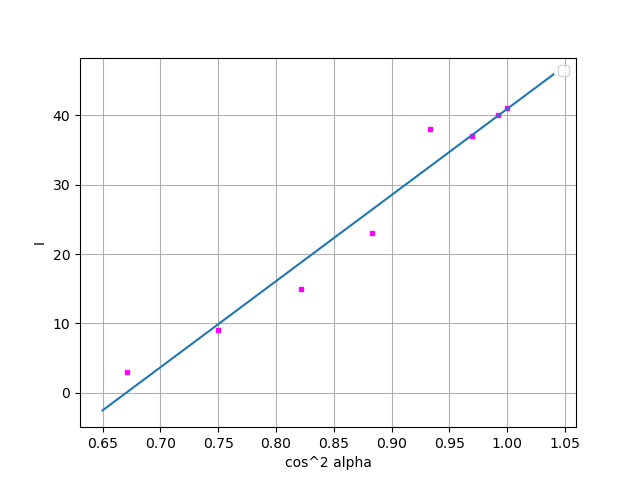
\includegraphics[scale=0.7]{graph1.png}
\centering
\caption{Зависимость интенсивности $I$ от угла $\alpha$}
\end{figure}

\subsection{Интерференция волн, отражённых от зеркала и решётки}

Закрепим на фиксаторах перед зеркалом металлическую решётку. Снимем зависимость интенсивности $I$ от координаты $x$ подвижного зеркала (Таблица 2). Построим график зависимости $I(x)$ (Рисунок 5).

Длина волны, определённая по этому графику - $\lambda_1 = 7,300 \pm 0,014$ мм. \par

Длина волны по частотогенератору: $\lambda_0 = 8,119 \pm 0,002$ мм (частота $\nu = 36,95\pm 0,01$ ГГЦ).

\begin{table}[h!]
\centering
\begin{tabular}{|l|r|r|r|r|r|}
\hline
\textbf{} & \multicolumn{1}{l|}{\textbf{I, мкВ}} & \multicolumn{1}{l|}{\textbf{x, мм}} & \multicolumn{1}{l|}{} & \multicolumn{1}{l|}{\textbf{I, мкВ}} & \multicolumn{1}{l|}{\textbf{x, мм}} \\ \hline
1 & 97 & 9,74 & 9 & 0 & 15,55 \\ \hline
2 & 55 & 10,45 & 10 & 25 & 16,33 \\ \hline
3 & 28 & 10,70 & 11 & 78 & 17,48 \\ \hline
4 & 0 & 12,15 & 12 & 73 & 17,76 \\ \hline
5 & 21 & 13,45 & 13 & 91 & 17,43 \\ \hline
6 & 80 & 14,45 & 14 & 50 & 17,96 \\ \hline
7 & 24 & 14,60 & 15 & 24 & 18,62 \\ \hline
8 & 43 & 14,11 & 16 & 0 & 19,45 \\ \hline
\end{tabular}
\caption{Интерференция на зеркале с решеткой}
\label{tab: 1}
\end{table}
    
\begin{figure}[h!]
    \centering
    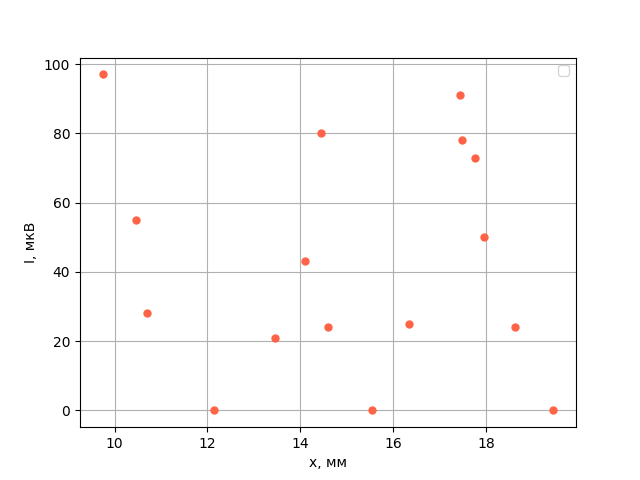
\includegraphics[width=14cm]{Figure_1.png}
    \caption{График зависимости интенсивности сигнала от координаты подвижного зеркала}
    \label{fig:vac}
\end{figure}


\subsection{Интерферометр Майкельсона}
\begin{enumerate}
    \item Соберём схему интерферометра Майкельсона согласно рис. 3, настроим установку на максимум сигнала. 
    \item Перемещая подвижное зеркало З2, снимем зависимость координаты $x_m$ в точке интерференционного максимума от номера максимума $m$, построим график зависимости $x_m = f(m)$. По графику определим длину волны: $\lambda_2 = 7,8 \pm  0,2$ мм.
    
\begin{table}[h!]
\centering
\begin{tabular}{|r|r|}
\hline
\multicolumn{1}{|l|}{\textbf{m}} & \multicolumn{1}{l|}{\textbf{x, мм}} \\ \hline
0 & 9,74 \\ \hline
1 & 14,45 \\ \hline
2 & 17,43 \\ \hline
3 & 20,32 \\ \hline
4 & 25,85 \\ \hline
5 & 29,49 \\ \hline
\end{tabular}%
\caption{Координаты максимумов}
\label{tab:my-table}
\end{table}
    
\begin{figure}[h]
    \centering
    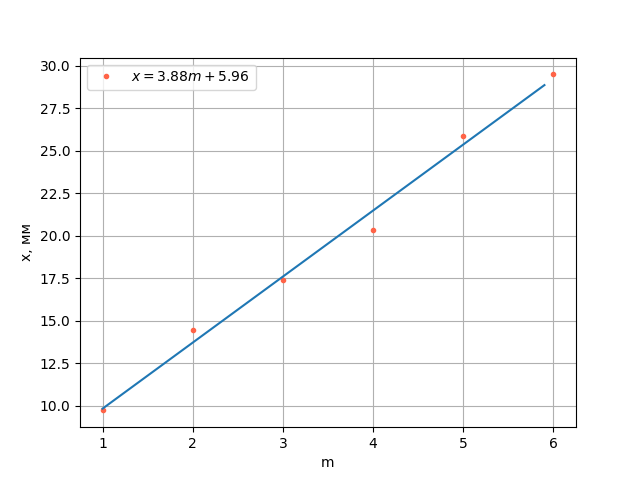
\includegraphics[width=10cm]{newgraph3.png}
    \caption{График зависимости координаты подвижного зеркала от номера интерференционного максимума}
    \label{fig:vac}
\end{figure}


\item Поместим перед подвижным зеркалом З2 тефлоновую пластину толщиной $3.2$ мм. Смещение интерференционного максимума от прежнего положения составляет $1,40$ мм. По формуле (5) определим показатель преломления тефлона: $n_1 = 1.438 \pm0.010 $. Табличное значение: $n_0  = 1.315$
\end{enumerate}
    
\section{Вывод}
В ходе работы была изучена интерференция электромагнитных волн миллиметрового диапазона с помощью оптических схем. Несколькими способами определена длина волны:
\begin{center}

    $\lambda_0 = 8,119 \pm 0,002$ мм  (частотогенератор) \par
    $\lambda_1 = 7,300 \pm 0,014$ мм (интерференция с решёткой) \par
    $\lambda_2 = 7,8 \pm  0,2$ мм (интерферометр Майкельсона)
\end{center}
Также был определен показатель преломления тефлона:
\begin{center}
    $n_{th} = 1.315$ \hspace{1cm}
    $n_1 = 1.438 \pm0.010 $
\end{center}

\end{document}